\section{Experimental Methodology}

\subsection{Research questions}

The evaluation addresses four research questions:
\begin{itemize}
\item \textbf{RQ1---False-safe twin behavior:} Can an OSPF candidate be control-plane consistent between the operational network and its twin while violating the operational latency SLO?
\item \textbf{RQ2---Residual-only gating:} Does a global residual-calibration policy retain useful acceptance under heterogeneous and shifted delay schedules?
\item \textbf{RQ3---Targeted drift sensing:} Does probing the candidate link before deployment improve latency prediction and the safety--utility trade-off?
\item \textbf{RQ4---Held-out evaluation after freezing:} Does the selected policy retain useful behavior on a randomized holdout that is not used for calibration or policy selection?
\end{itemize}

The experiment is designed as a controlled causal study rather than a production-scale benchmark. The manipulated variable is the hidden per-direction latency on the operational candidate link; the twin topology, routing configuration, candidate configuration, and host workloads are held constant.

\subsection{Execution environment}

Experiments run on an Apple-silicon MacBook Pro using an Ubuntu machine provided by OrbStack. Containerlab version 0.77.0 orchestrates the network containers. Routers use \texttt{quay.io/frrouting/frr:10.5.1}; end hosts use \texttt{wbitt/network-multitool:3.22.2}. The operational laboratory is named \texttt{ospf-ops}, and the twin laboratory is named \texttt{ospf-twin}. Each environment runs independently so that operational impairments do not modify the twin.

\begin{figure}[t]
\centering
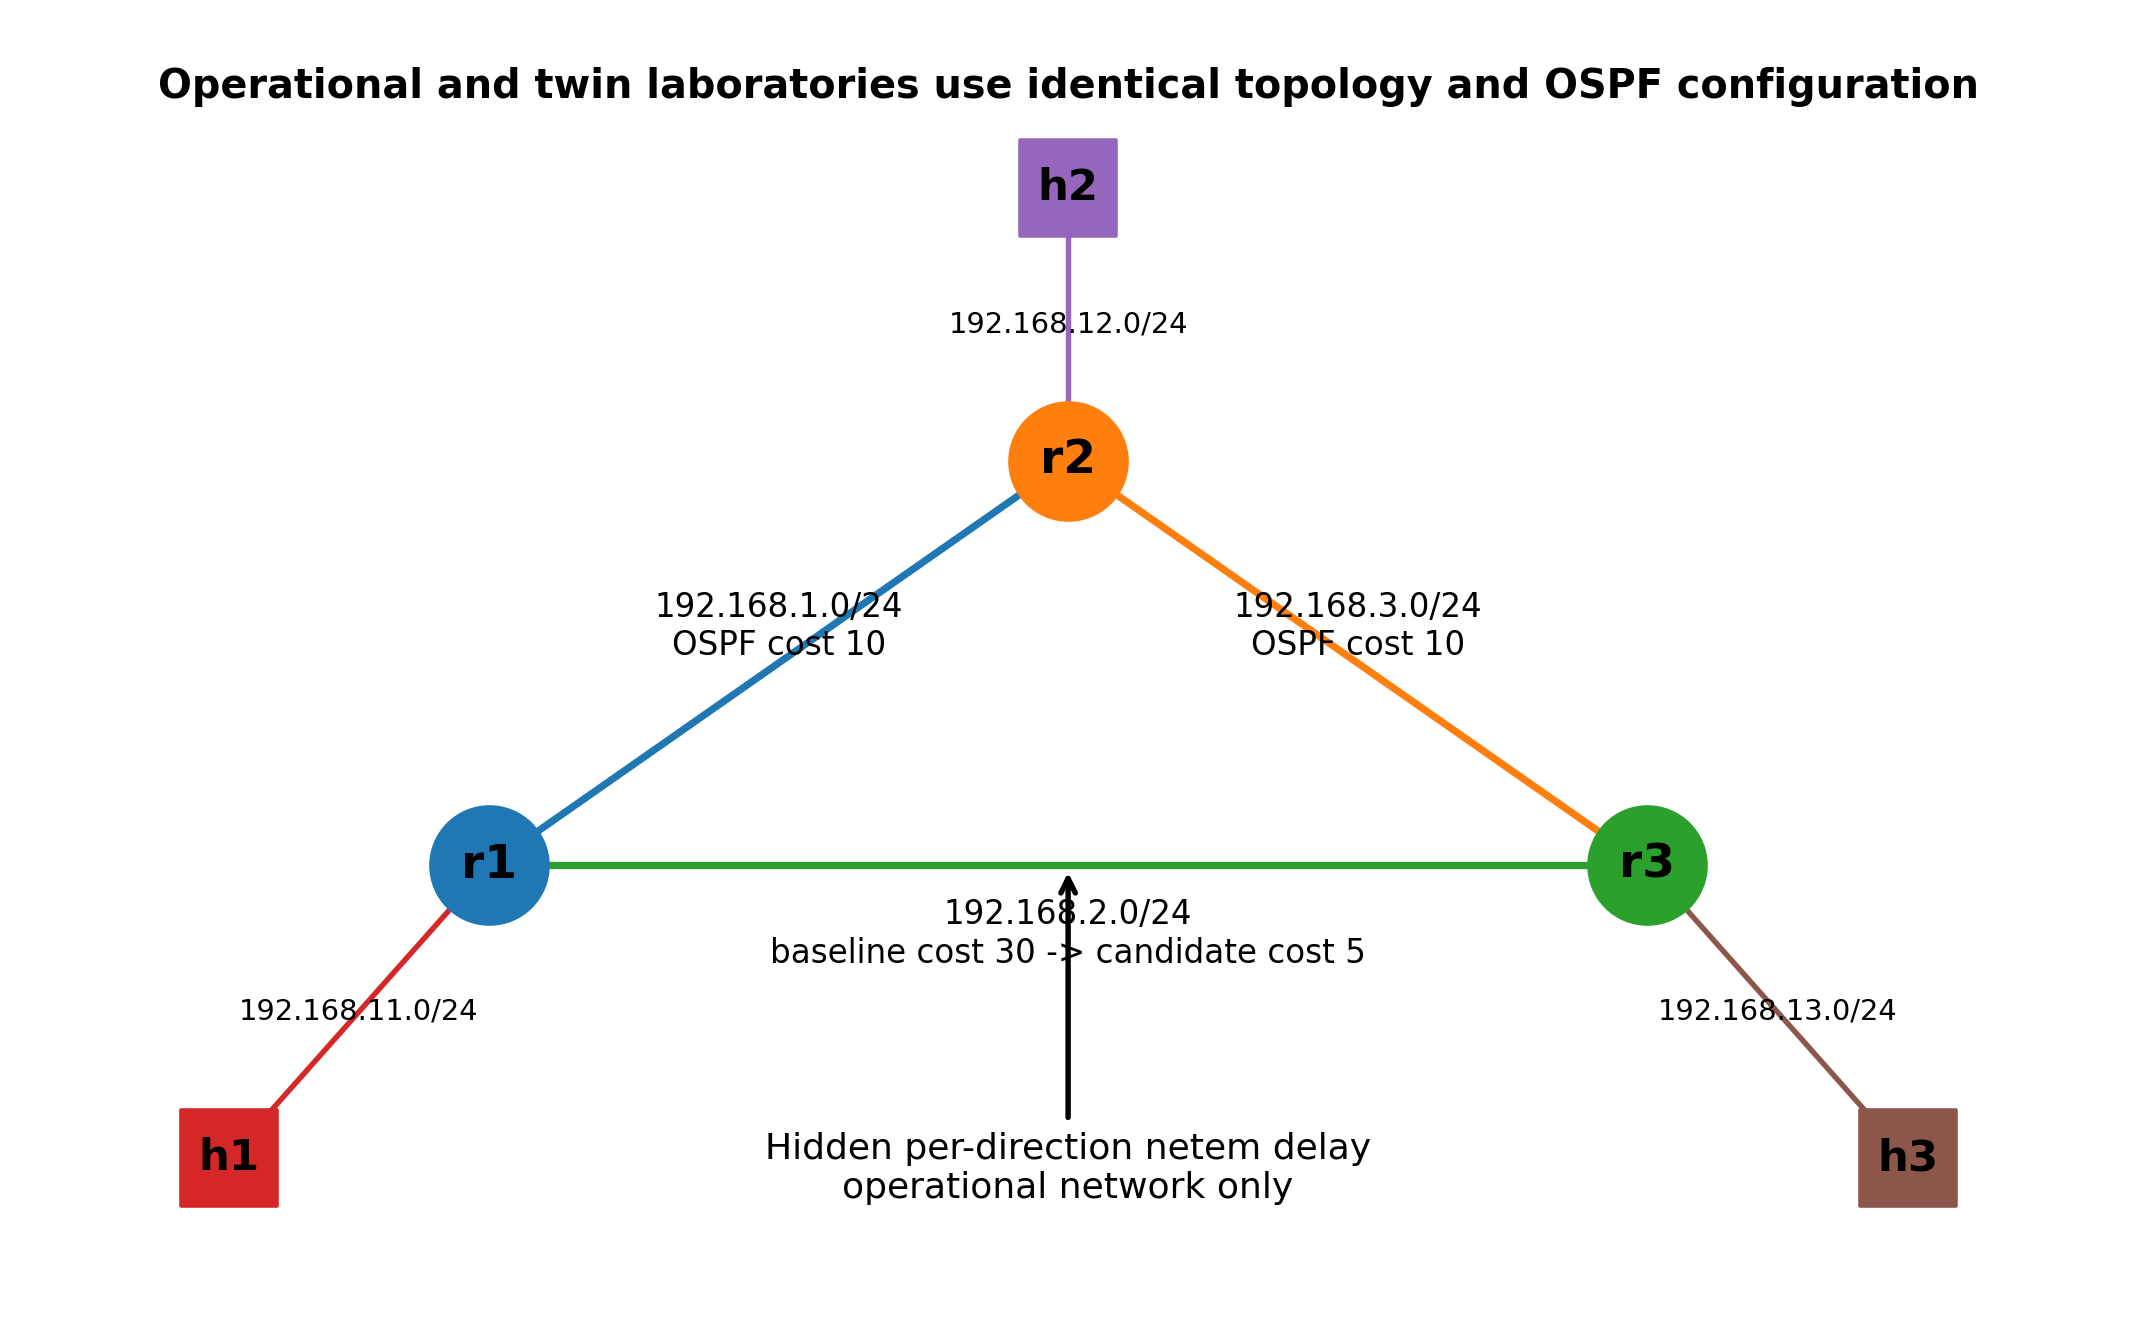
\includegraphics[width=\columnwidth]{figures/figure0_testbed_topology.png}
\caption{Experimental topology shared by the operational and twin laboratories. Hidden \texttt{netem} delay is applied only to the operational $r_1$--$r_3$ candidate link.}
\label{fig:topology}
\end{figure}

\subsection{Network topology}

Each environment contains three FRRouting routers arranged in a triangle, with one host attached to each router. The number on each router-to-router edge denotes the baseline OSPF cost. Host $h_2$ is attached to $r_2$, although the primary measured flow is $h_1\rightarrow h_3$.

The candidate changes the direct $r_1$--$r_3$ cost from 30 to 5 on both ends. The baseline route from $r_1$ to the LAN behind $r_3$ uses $r_2$ and has metric 30. The candidate route uses the direct link and has metric 15, including the destination-interface cost.

Before each schedule, a readiness script confirms that both laboratories are deployed; every expected OSPF adjacency is in the Full/- state; the destination route is installed; and $h_1$ can reach $h_3$.

\subsection{Controlled drift injection}

The operational candidate link is the direct $r_1$--$r_3$ connection. The experiment applies Linux \texttt{netem} delay to the corresponding interface on both operational endpoints. The twin receives no delay modification.

The per-direction delay levels are
\[
D=\{0,1,2,5,10,15,20,25,30,35,40\}\text{ ms}.
\]
Applying delay in both directions produces an approximate round-trip contribution of $2d$, with normal container and host-scheduling variation.

For each sample, the harness first sets the requested delay and returns OSPF to the baseline cost state. After the sample has been parsed, the next sample sets its own delay and baseline state. At the end of a schedule, delay is reset to zero and the baseline costs are restored.

\subsection{Per-sample protocol}

Each sample executes the following sequence:
\begin{enumerate}
\item apply the operational delay level;
\item set operational and twin OSPF costs to the baseline state;
\item send 20 ICMP probes from operational $r_1$ to operational \texttt{192.168.2.2};
\item send the corresponding 20 probes in the twin;
\item set both environments to the candidate OSPF state;
\item record the installed route to \texttt{192.168.13.0/24} in both environments;
\item send 20 end-to-end ICMP probes from $h_1$ to $h_3$ in each environment; and
\item parse the measurements into a structured sample summary.
\end{enumerate}

Pings use an interval of 0.1 s and a response timeout of 2 s. The parser records packet-loss percentage and minimum, mean, maximum, and variation of RTT. FRRouting's BusyBox-style three-value link-probe summary is supported by treating the missing variation field as zero.

The scripts do not override ICMP payload size, so each container's default ping payload is used. No warm-up request or first reply is discarded: the reported mean is the summary mean over all received replies from the 20 requests. The candidate-state script waits 2 s after updating the OSPF cost on both endpoints before route and end-to-end measurements are collected.

The direct link probes occur before the operational candidate is applied. The post-change operational end-to-end measurement is collected only to construct ground truth for evaluation. It is not an input to the deploy/reject rule.

\subsection{Dataset partitions}

\textbf{Calibration:} \texttt{calibration\_seed77} contains 22 samples: two observations for each of the 11 delay levels, randomized using seed 77. These samples determine the fixed one-sided residual margin.

\textbf{Validation:} Policy selection uses 186 validation samples from five schedules. The three randomized schedules expose the policy to order variation while preserving the same delay support. The abrupt-shift and up/down schedules test whether policy utility depends on a stationary or smoothly ordered sequence.

\textbf{Holdout:} \texttt{holdout\_seed909} contains 33 samples: three observations for each of the 11 delay levels in a randomized order generated with seed 909. The holdout is not used to compute the margin, compare candidate policies, or select a policy. The policy manifest fixes the method, SLO, calibration size, order-statistic rank, residual margin, prediction rule, and deployment rule before holdout evaluation.

\subsection{Experimental phases}

The artifact records the development process as separate phases.

\textbf{Phase 1---convergence smoke test:} The first phase verifies that the three-router OSPF laboratory converges and that changing the direct-link cost moves traffic to the intended route.

\textbf{Phase 2---first false-safe twin case:} A hidden 30 ms per-direction delay is applied to the operational direct link. After the candidate OSPF change, both environments select the direct route. The twin predicts a sub-millisecond RTT, whereas the operational RTT is about 66 ms and violates the 50 ms SLO. This establishes RQ1.

\textbf{Phase 3---delay sweep and preliminary gates:} A 55-sample delay sweep explores the relation between injected delay, operational RTT, twin error, and residual-based gates. This phase is exploratory and is not used as the final holdout.

\textbf{Phase 4---residual-only policy validity:} A 22-sample calibration set and 186 validation samples evaluate static and rolling residual policies. The static policy and rolling windows of 20 and 50 observations reject every candidate. The rolling window of 10 observations is non-vacuous but admits two unsafe changes and fails the cross-schedule utility criterion. These results motivate method revision.

\textbf{Phase 5---candidate-link sentinel:} The candidate-link sentinel uses the same schedule definitions and the same 22/186 calibration-validation sizes, but Phase 5 is an independent measurement run rather than a reuse of Phase 4 records. The calibrated sentinel is selected and frozen before the 33-sample holdout is evaluated once.

\subsection{Compared policies}

Four policies are evaluated from the same sample records:
\begin{itemize}
\item \textbf{Direct:} deploy every candidate.
\item \textbf{Twin only:} deploy when twin end-to-end RTT is at most 50 ms.
\item \textbf{Raw sentinel:} deploy when the corrected prediction is at most 50 ms.
\item \textbf{Conformal sentinel:} deploy when the corrected prediction plus the frozen 0.661 ms margin is at most 50 ms.
\end{itemize}
Using common sample records permits paired comparison. Every policy receives the same pre-deployment observables and ground-truth label.

\subsection{Policy-selection protocol}

Candidate policies are compared only on calibration and validation data. A policy is ineligible when it accepts no candidates, accepts no safe candidate, or fails to accept at least one safe candidate in every validation schedule. Among eligible policies, selection is lexicographic: minimize unsafe deployments; maximize safe-change coverage; and maximize total acceptance. This protocol explicitly rejects complete abstention as a misleading safety result.

The selected conformal candidate-link sentinel is recorded in \texttt{frozen\_policy.json} with calibration size 22, $\alpha=0.05$, finite-sample rank 22, margin 0.661 ms, latency SLO 50 ms, the exact prediction and deployment rules, and SHA-256 hashes of the validation inputs.

\begin{table*}[t]
\caption{Validation schedules and their experimental purpose.}
\label{tab:schedules}
\centering
\scriptsize
\begin{tabularx}{\textwidth}{l r X}
\toprule
Schedule & Samples & Design purpose\\
\midrule
\texttt{randomized\_seed101} & 33 & Three randomized repetitions of each delay\\
\texttt{randomized\_seed202} & 33 & Independent randomized ordering\\
\texttt{randomized\_seed303} & 33 & Independent randomized ordering\\
\texttt{abrupt\_shift} & 45 & Low-delay regime, abrupt high-delay regime, then recovery\\
\texttt{up\_down} & 42 & Repeated ascending and descending delay sweeps\\
\midrule
Total & 186 & \\
\bottomrule
\end{tabularx}
\end{table*}

\subsection{Holdout execution and incident disclosure}

The holdout runner checks that the frozen-policy manifest exists and that no completed holdout-results file is present. It refuses a second evaluation after \texttt{holdout\_results.json} has been created.

During the first holdout sample, raw measurements were collected before the policy manifest had been committed because the results directory was ignored by the initial \texttt{.gitignore}. Parsing then stopped because the link probe used a three-value BusyBox ping summary rather than the four-value format expected by the parser.

The raw first-sample files were preserved. The parser was modified only to accept both ping formats, and the existing measurements were parsed without remeasurement. No margin, SLO, policy rule, schedule, or sample value was changed. The policy file and parser correction were committed in a new commit, and the holdout runner skipped the completed first summary before collecting the remaining 32 samples. The incident is disclosed in \texttt{docs/holdout\_execution\_log.md}.

This sequence means the first measurement preceded the Git commit containing the manifest, although the policy parameters already existed in the file and were not modified after measurement. The holdout was not used for calibration or policy selection; this procedural deviation is reported transparently.

\subsection{Outcome variables}

The primary policy outcomes are:
\begin{itemize}
\item accepted candidates;
\item unsafe deployments;
\item unsafe rate among accepted candidates;
\item safe accepted candidates;
\item safe rejected candidates;
\item safe-change coverage; and
\item acceptance rate.
\end{itemize}

Prediction quality is reported using:
\begin{itemize}
\item mean absolute error;
\item root mean squared error;
\item corrected residuals; and
\item Pearson correlation between corrected prediction and observed RTT.
\end{itemize}
The experiment also checks route agreement between the operational network and twin.

\subsection{Statistical reporting}

For proportions, the analysis reports 95\% Wilson confidence intervals. A zero observed unsafe count is not reported as proof of zero true risk.

The conformal upper score is separately evaluated as a predictive bound. This distinguishes:
\begin{enumerate}
\item binary deployment-classification performance relative to the 50 ms SLO; and
\item empirical coverage of realized RTT by the upper score.
\end{enumerate}
This distinction is necessary because the holdout decisions were all correct, while the nominal 95\% upper-bound coverage was not achieved.

\subsection{Integrity and reproducibility controls}

The artifact uses the following controls:
\begin{itemize}
\item generated schedules are stored as CSV files;
\item processed rows preserve sample ID, schedule, position, delay, repetition, role, and seed;
\item validation and holdout results are stored as JSON;
\item the policy manifest records source hashes;
\item holdout-result files prevent automatic second execution;
\item dated provenance records separate policy freezing, holdout completion, evaluator correction, and final analysis;
\item analysis files record the parser incident and evaluator correction; and
\item the final holdout dataset is checked for 33 unique IDs, positions 1--33, three repetitions per delay, consistent safety labels, and universal route agreement.
\end{itemize}
